\documentclass[11pt,a4paper]{article}
\usepackage[utf8]{inputenc}
\usepackage[margin=0.85in]{geometry}
\usepackage{graphicx}
\usepackage{hyperref}
\usepackage{booktabs}
\usepackage{caption}
\usepackage{float}
\usepackage{enumitem}

\hypersetup{
    colorlinks=true,
    linkcolor=blue,
    filecolor=magenta,      
    urlcolor=cyan,
    pdftitle={Design Document using SA/SD Methodology: Website Vulnerability Scanner},
    pdfpagemode=UseOutlines,
}

\title{\textbf{Data Flow Diagram}\\ \Large for\\ \textbf{Website Vulnerability Scanner}}
\author{%
  \textbf{Prepared by}\\[0.5em]
  Deepthi K (241IT021)\\
  Jasmine (241IT051)\\
  Sacheth Koushal (241IT058)\\[1.2em]
  \textbf{Department of Information Technology}\\
  \textbf{National Institute of Technology Karnataka, Surathkal}
}
\date{August 2026}

\begin{document}

\maketitle

\tableofcontents
\newpage

\section{Data Flow Diagram (DFD) Model}

\subsection{Level 0 DFD}
\subsubsection{Context Diagram}

Figure \ref{fig:level0} shows the Level 0 Context Diagram for the Website Vulnerability Scanner system. It defines the main system boundary for Process 0 and models all inbound/outbound interaction channels with main external entities such as the WVS User, System Administrator, Target Website, Public DNS Resolvers, SMTP Relay, and OSV/EPSS Advisory APIs.

\begin{figure}[H]
    \centering
    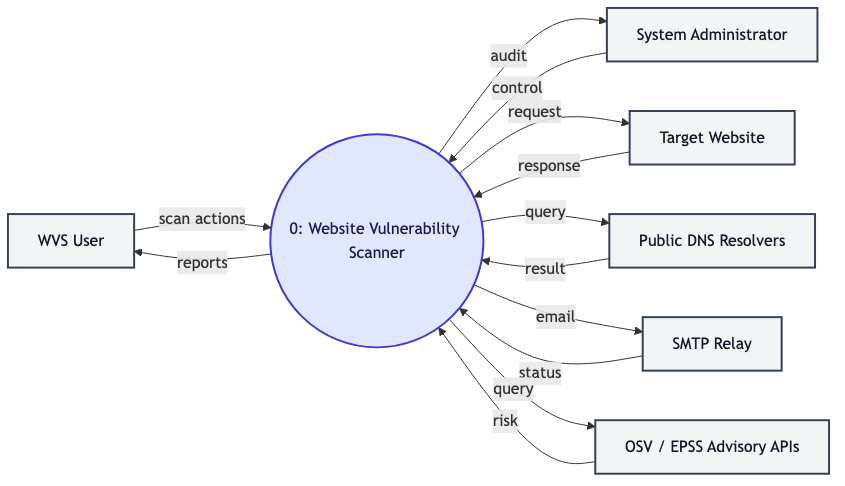
\includegraphics[width=0.88\textwidth,height=0.48\textheight,keepaspectratio]{mermaid/png/level-0.png}
    \caption{Level 0 Context Diagram}
    \label{fig:level0}
\end{figure}

\subsection{Level 1 DFD}
\subsubsection{Top-Level Functional Decomposition}

Figure \ref{fig:level1} shows the Level 1 DFD. Process 0 is decomposed into 8 primary functional modules ($0.1$ through $0.8$). It displays the main scanning pipeline from the initial user request through scope validation, discovery crawling, vulnerability detection, findings management, and report generation, as well as centralized Scope Guard enforcement ($0.8$) and third-party integrations.

\begin{figure}[H]
    \centering
    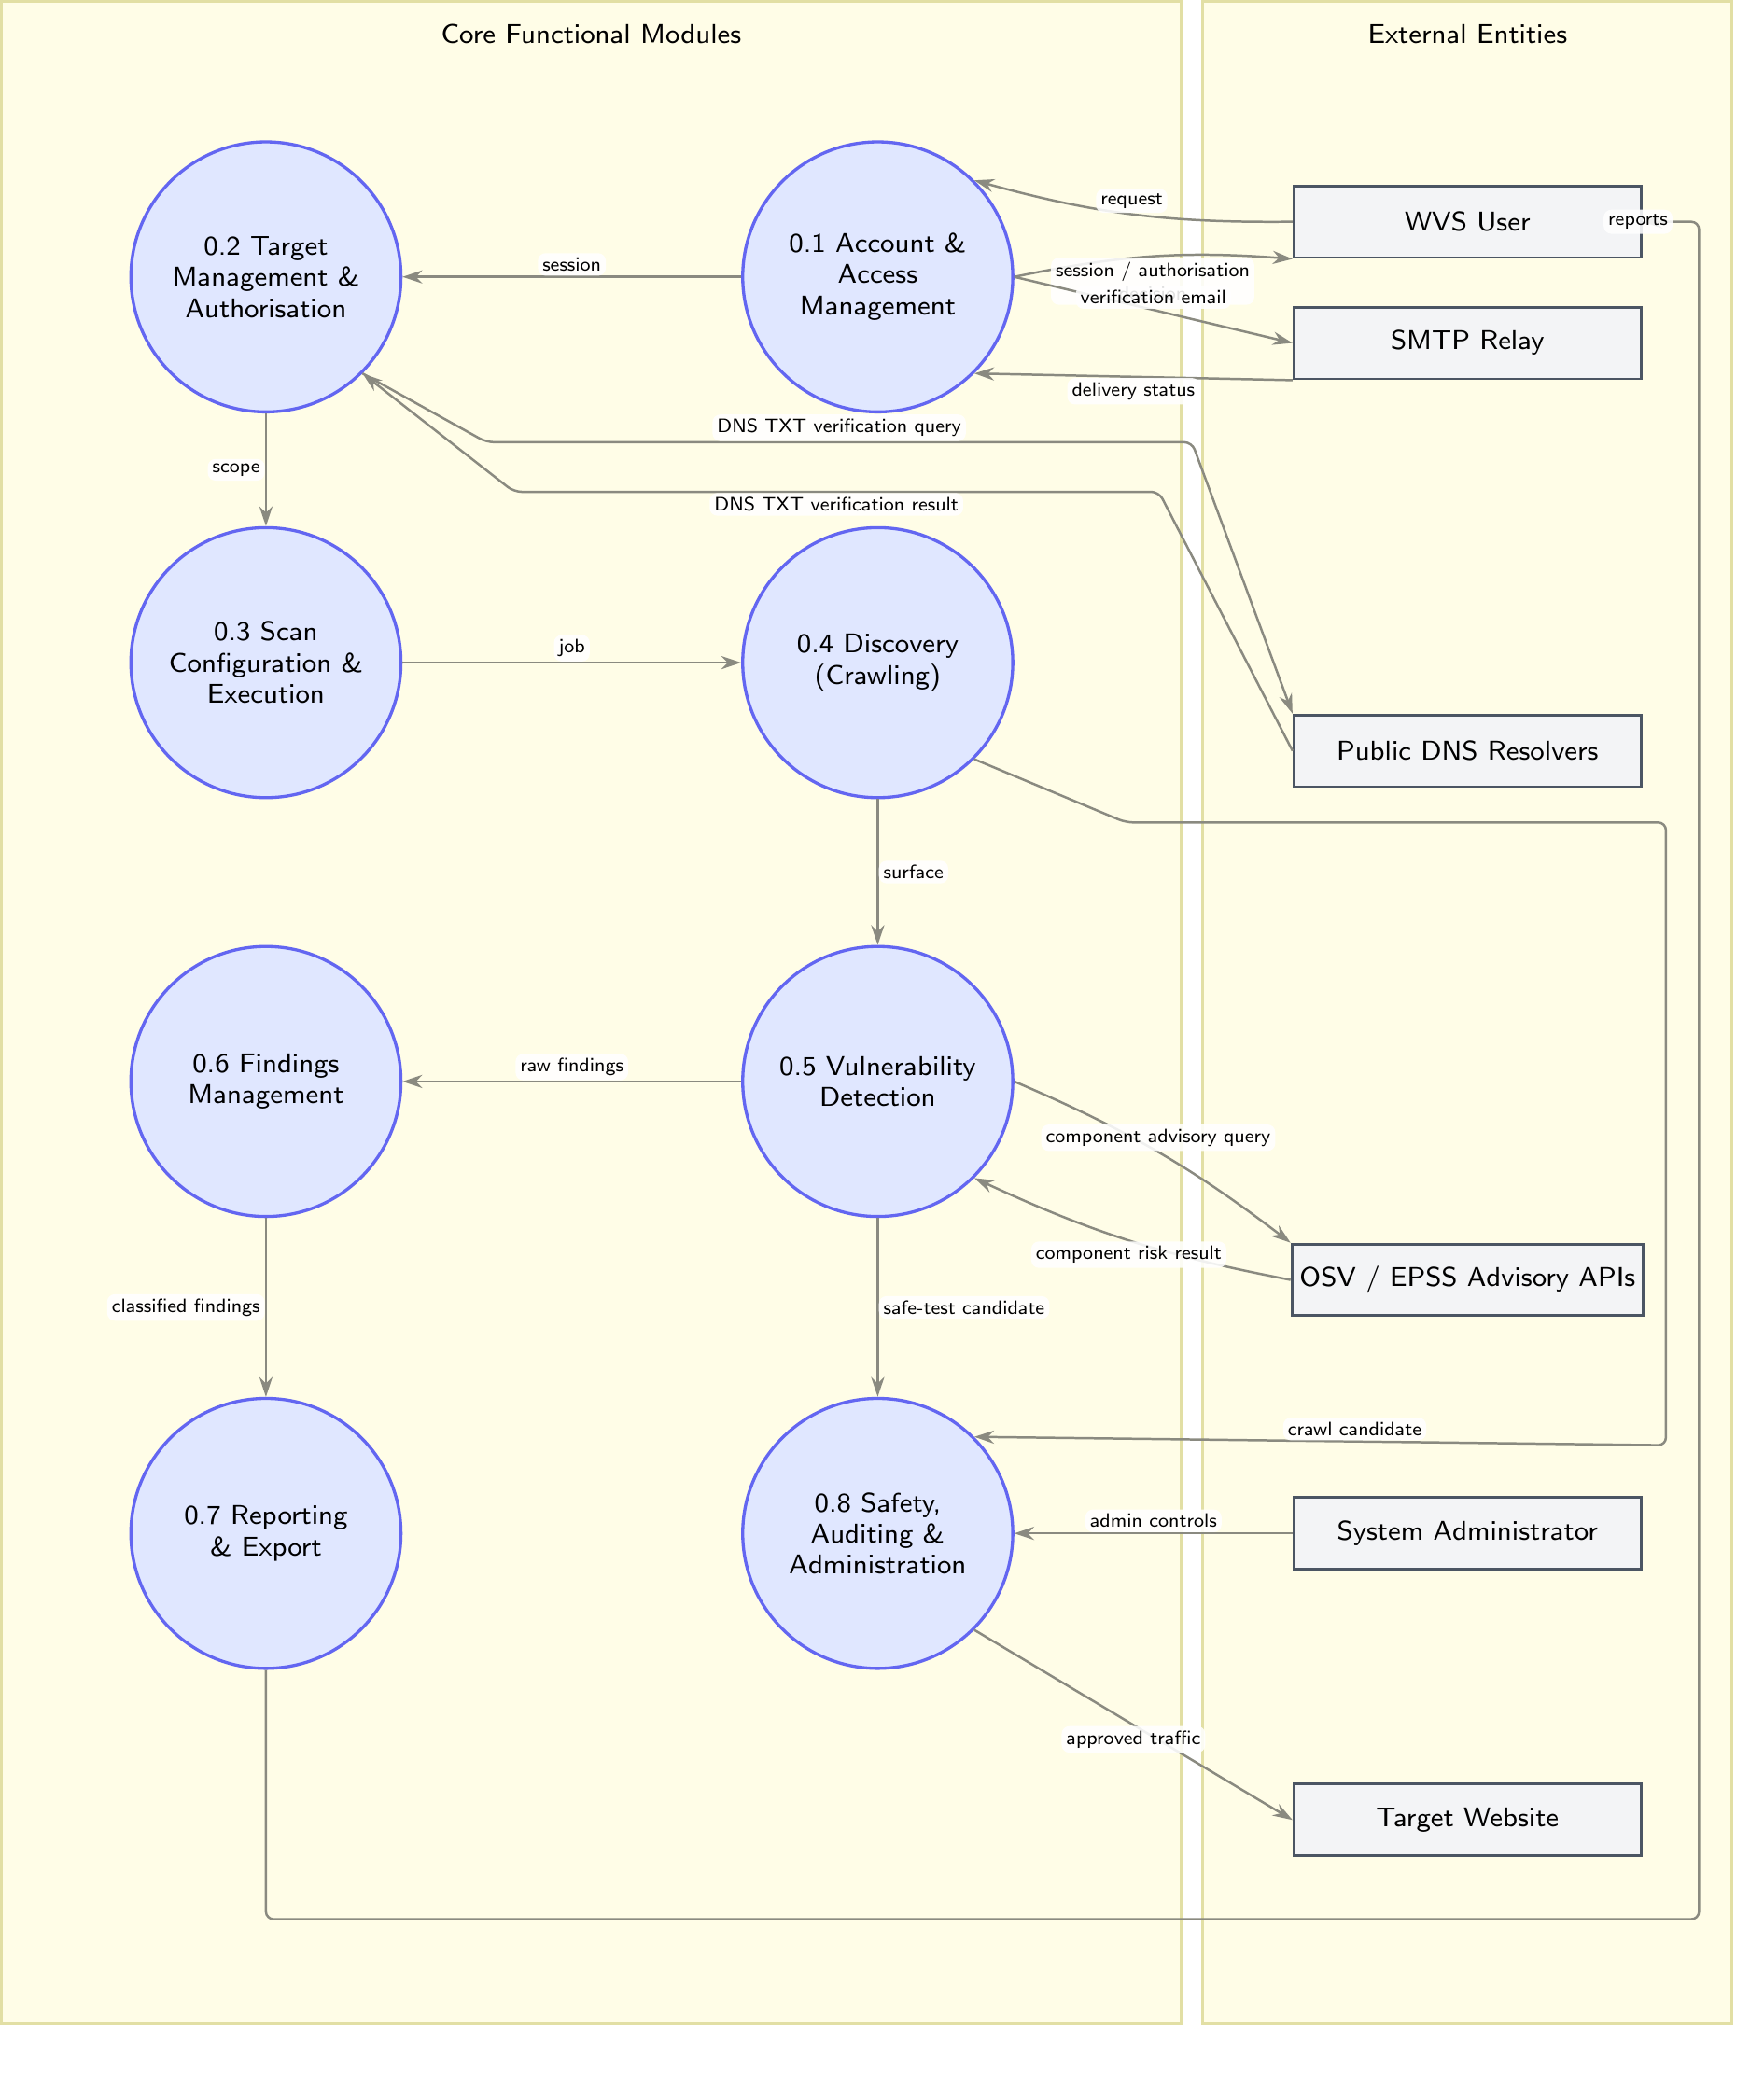
\includegraphics[width=0.94\textwidth,height=0.85\textheight,keepaspectratio]{mermaid/png/level-1.png}
    \caption{Level 1 DFD with 8 functional groups}
    \label{fig:level1}
\end{figure}
\newpage
\subsection{Level 2 DFDs}

\subsubsection{0.1 User Authentication \& Access Control}

Process $0.1$ is decomposed into credential validation, session token issuance, and login audit logging. Process 0.1.1 validates the user credentials by sending a verification request to Process 0.1.2 and saves the account and failed attempts in Data Store D1, Process 0.1.2 then issues session tokens and verifies email deliverability via SMTP Relay, and Process 0.1.3 records authentication audits.

\begin{figure}[H]
    \centering
    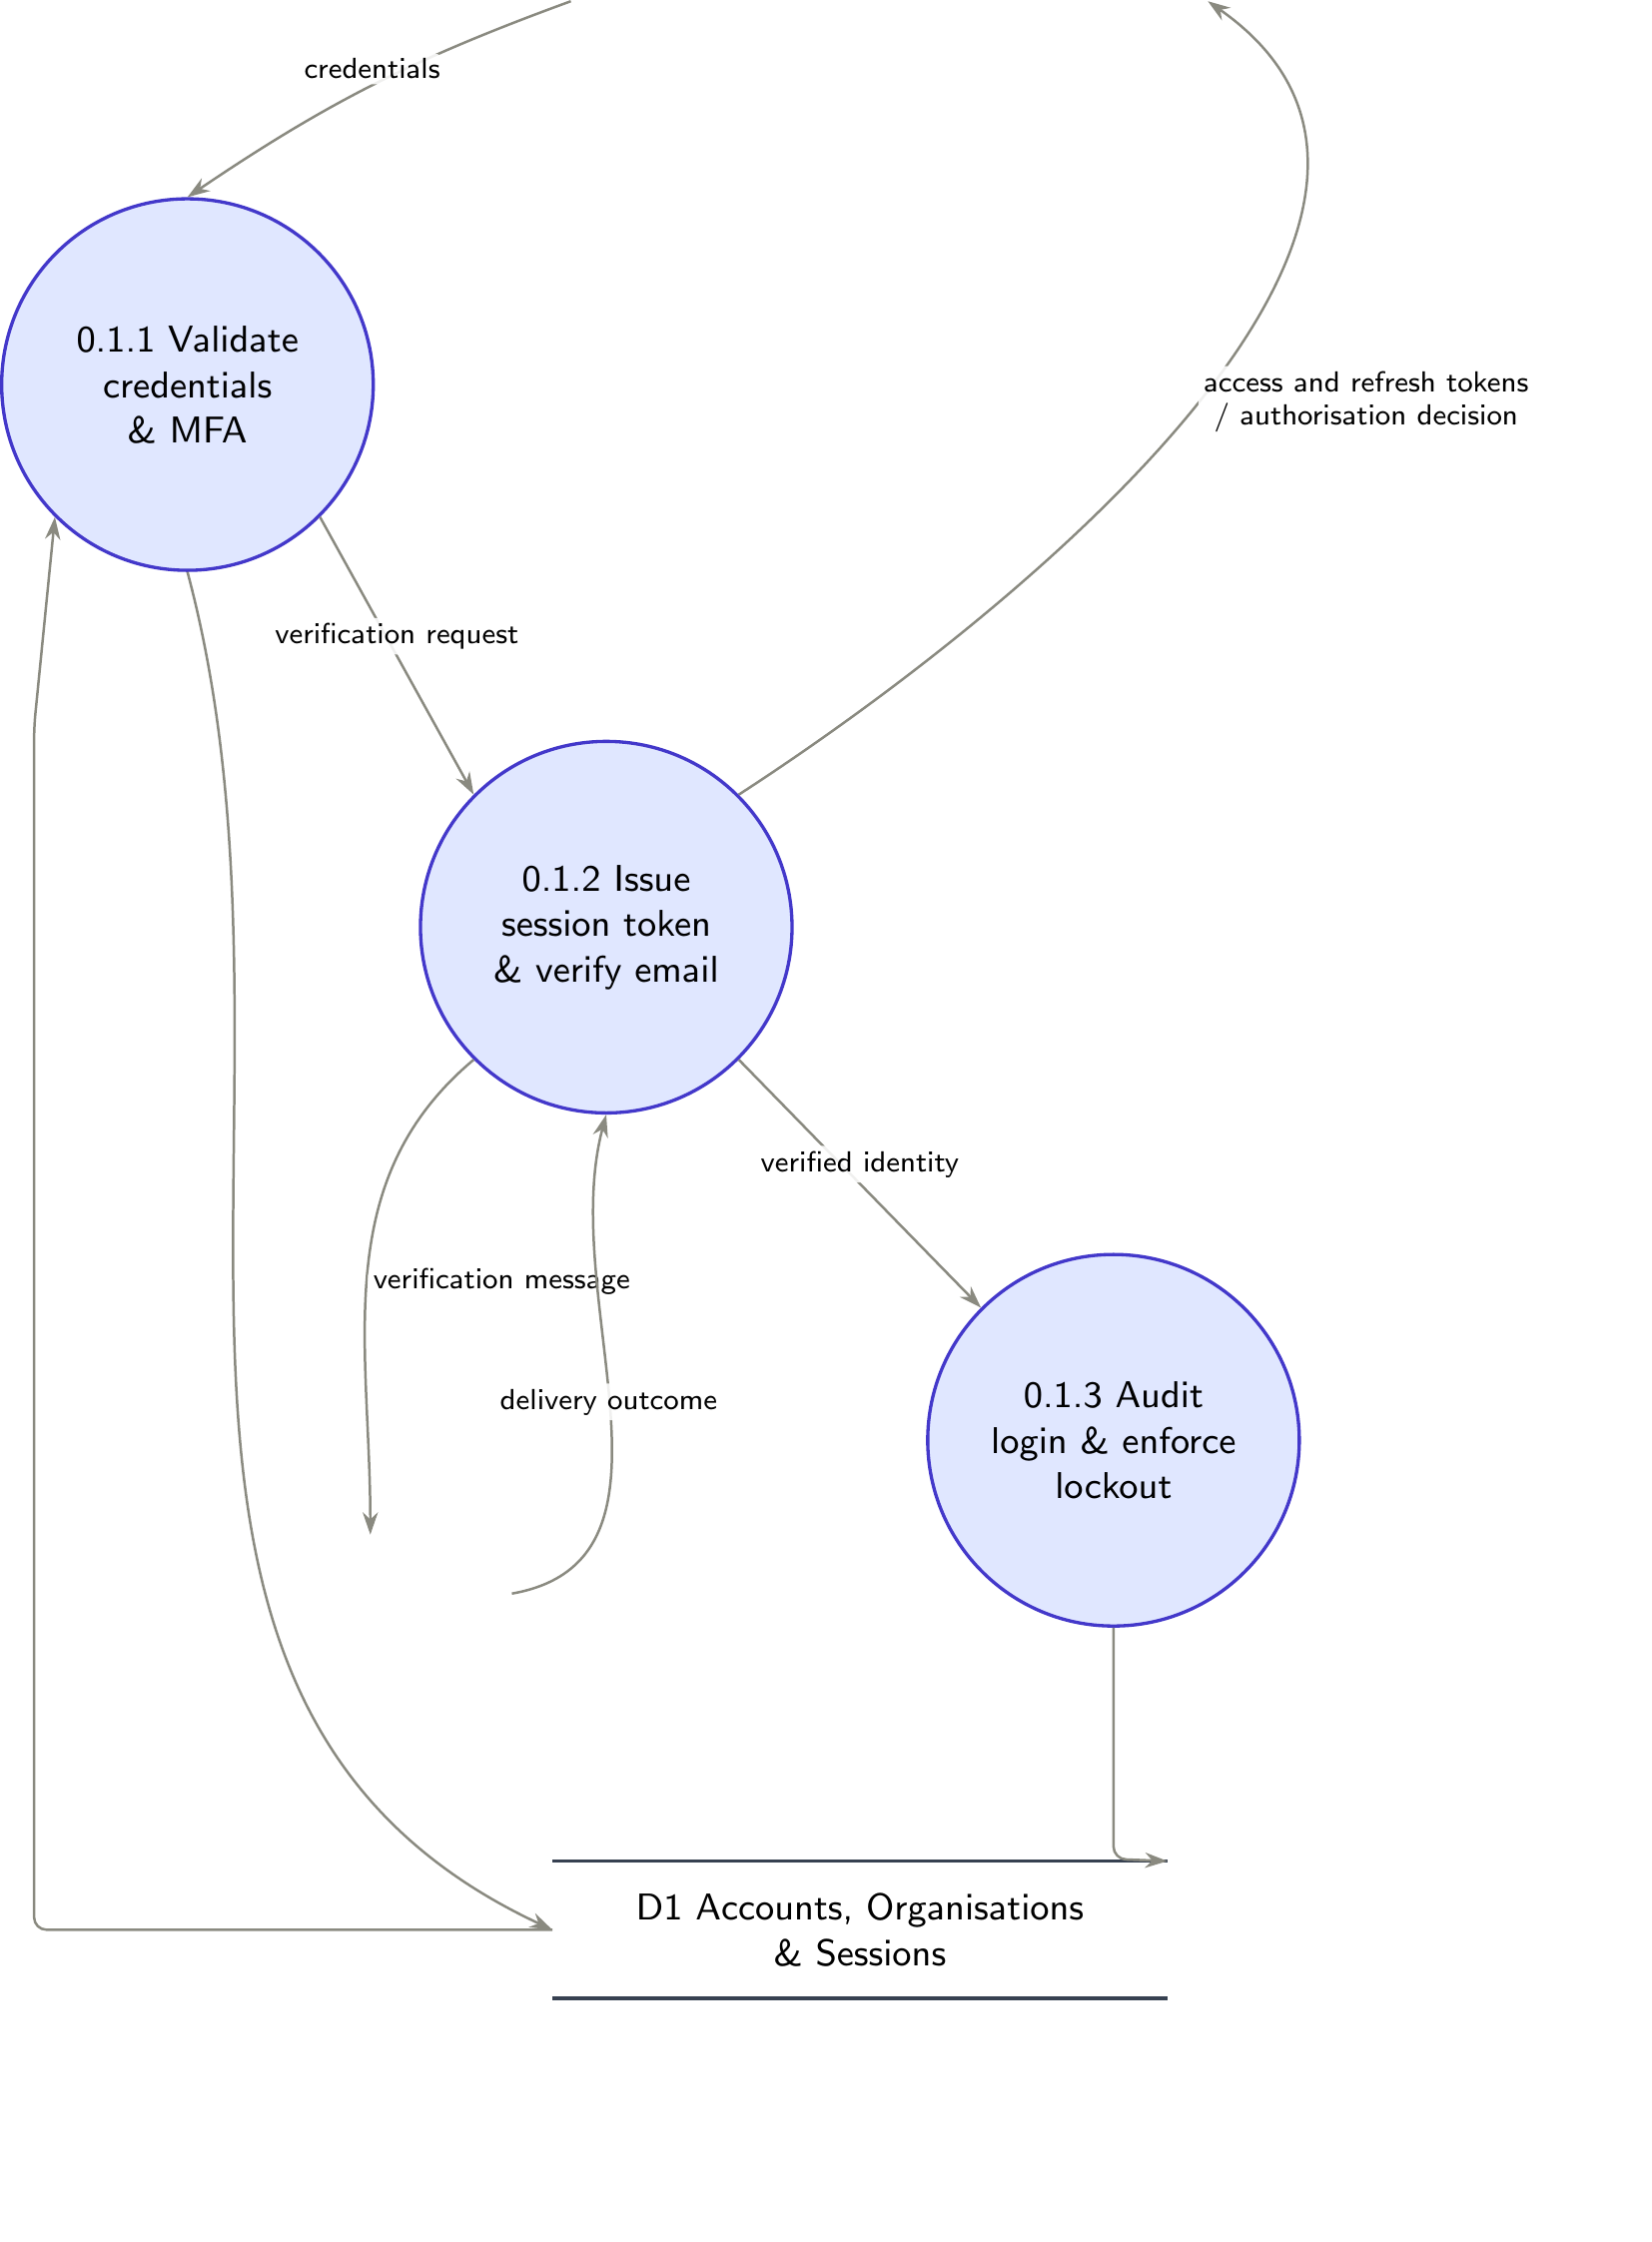
\includegraphics[width=0.94\textwidth,height=0.75\textheight,keepaspectratio]{mermaid/png/f.1.png}
    \caption{Level 2 DFD for 0.1 User Authentication \& Access Control}
    \label{fig:f1}
\end{figure}

\subsubsection{0.2 Target Management \& Authorisation}

Process $0.2$ is decomposed into target registration, verification token generation, and DNS/well-known proof validation. Process 0.2.1 registers target records in D2, Process 0.2.2 issues verification tokens for TXT/well known path validation and Process 0.2.3 validates these tokens against Public DNS and the Target Website.

\begin{figure}[H]
    \centering
    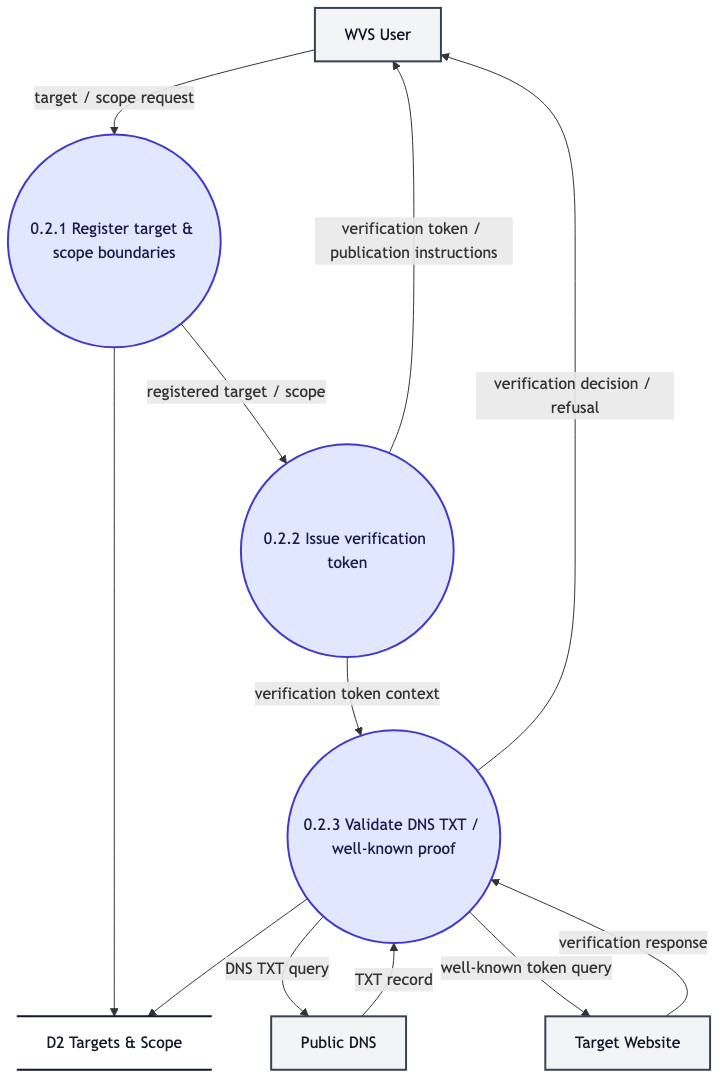
\includegraphics[width=0.94\textwidth,height=0.75\textheight,keepaspectratio]{mermaid/png/f.2.png}
    \caption{Level 2 DFD for 0.2 Target Management \& Authorisation}
    \label{fig:f2}
\end{figure}

\newpage
\subsubsection{0.3 Scan Configuration \& Execution}

Process $0.3$ is decomposed into scan profile validation, job scheduling, and lifecycle execution. Process 0.3.1 verifies user scope and quotas against D2 and Process 0.3.2 queues scan jobs in D3, and Process 0.3.3 executes the scan lifecycle while writing reproducibility records to D4.

\begin{figure}[H]
    \centering
    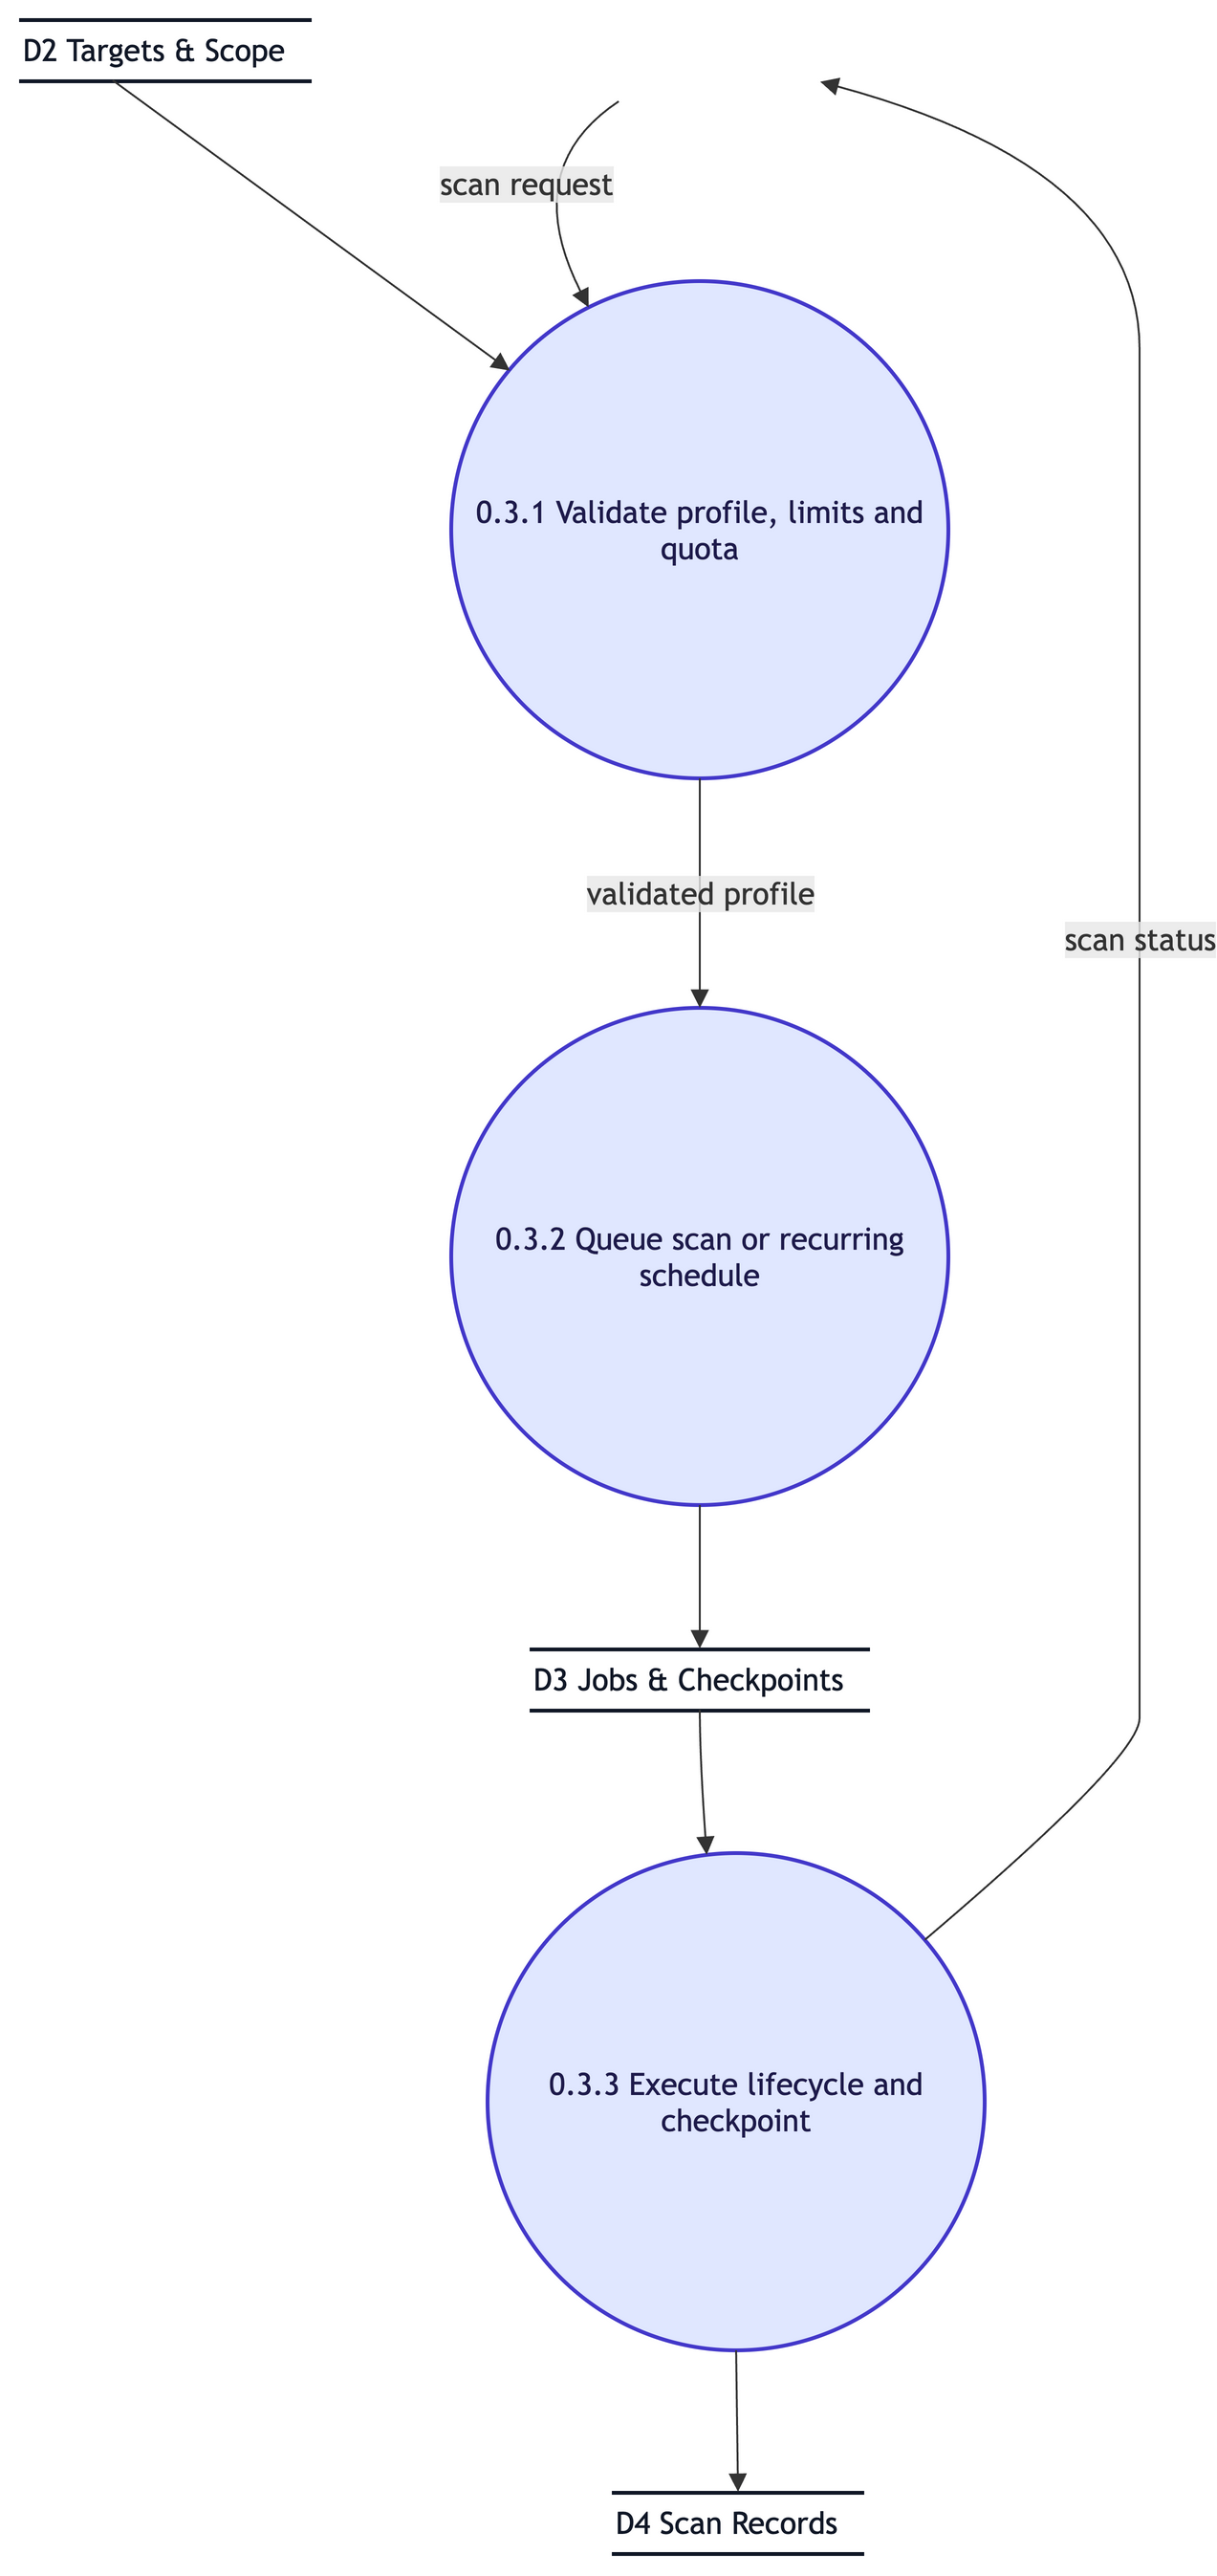
\includegraphics[width=0.94\textwidth,height=0.75\textheight,keepaspectratio]{mermaid/png/f.3.png}
    \caption{Level 2 DFD for 0.3 Scan Configuration \& Execution}
    \label{fig:f3}
\end{figure}

\subsubsection{0.4 Discovery (Crawling)}

Process $0.4$ is decomposed into scope loading, link/form discovery, and JS rendering deduplication. Process 0.4.1 loads ceilings from D2, Process 0.4.2 sends crawl candidates to Process 0.8 Scope Guard, and Process 0.4.3 records page inventory in D4 upon receiving HTTP responses from the Target Website.

\begin{figure}[H]
    \centering
    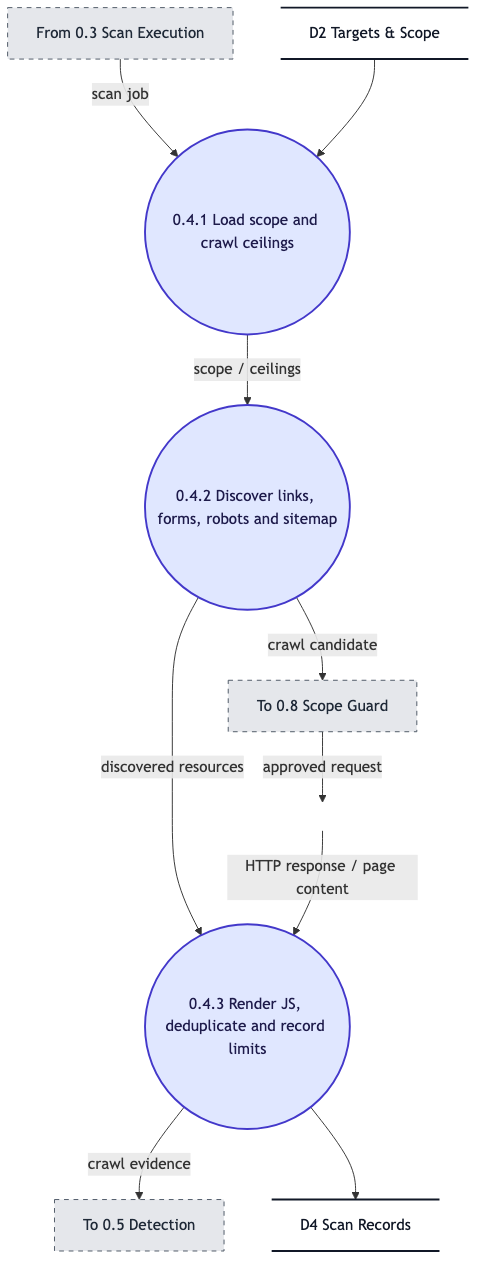
\includegraphics[width=0.94\textwidth,height=0.75\textheight,keepaspectratio]{mermaid/png/f.4.png}
    \caption{Level 2 DFD for 0.4 Discovery (Crawling)}
    \label{fig:f4}
\end{figure}

\newpage
\subsubsection{0.5 Vulnerability Detection}

Process $0.5$ is decomposed into passive header checking, safe active test preparation, and advisory version enrichment. Process 0.5.1 runs passive analysis, Process 0.5.2 routes active test payloads through Process 0.8 Scope Guard, and Process 0.5.3 queries OSV/EPSS APIs and stores evidence in D5.

\begin{figure}[H]
    \centering
    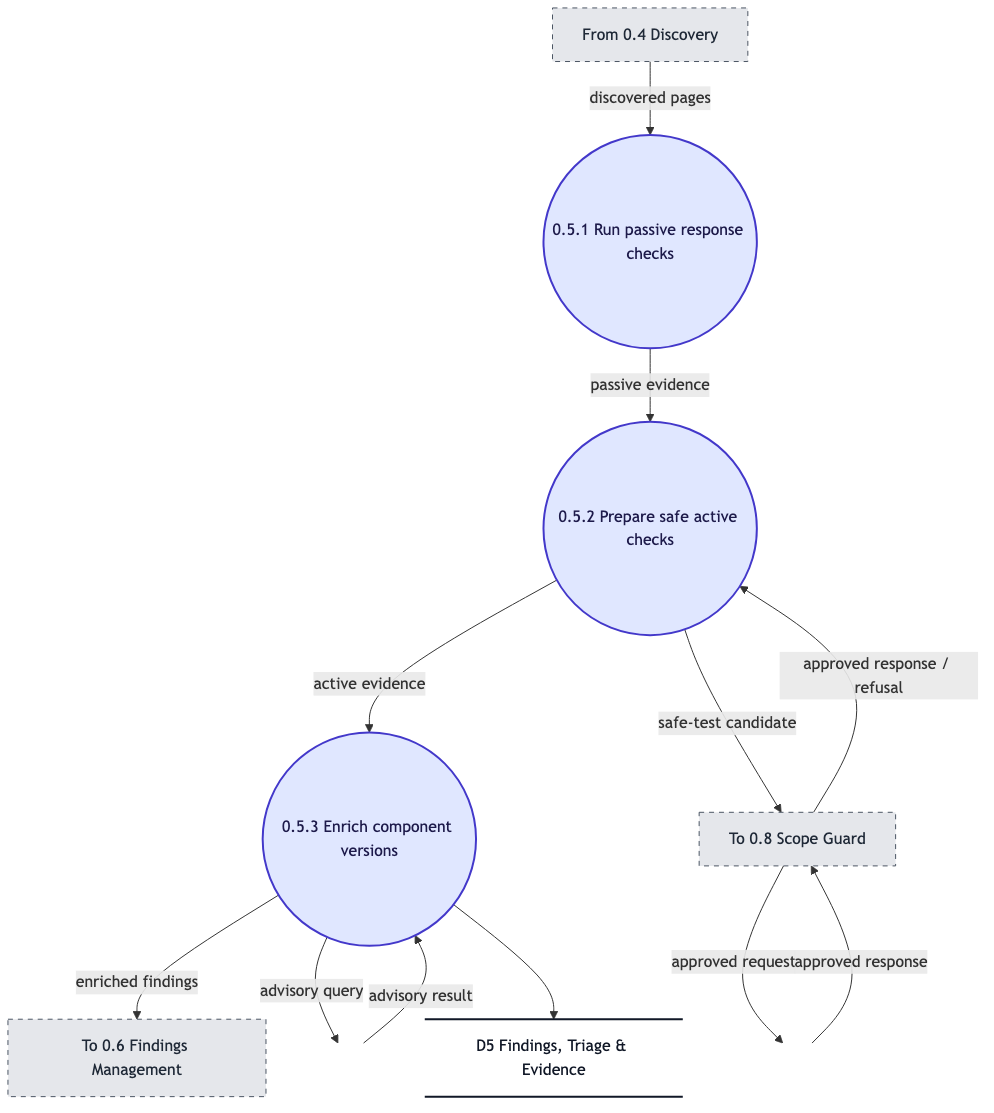
\includegraphics[width=0.94\textwidth,height=0.75\textheight,keepaspectratio]{mermaid/png/f.5.png}
    \caption{Level 2 DFD for 0.5 Vulnerability Detection}
    \label{fig:f5}
\end{figure}

\subsubsection{0.6 Findings Management}

Process $0.6$ is decomposed into normalisation/redaction, prior scan comparison, evidence retention and triage filtering. Process 0.6.1 ingests raw findings, normalises, redacts and deduplicates them. Process 0.6.2 compares prior scans stored in D5 and retains evidence, and Process 0.6.3 applies user triage, filters and sorts them and also implements severity classification.

\begin{figure}[H]
    \centering
    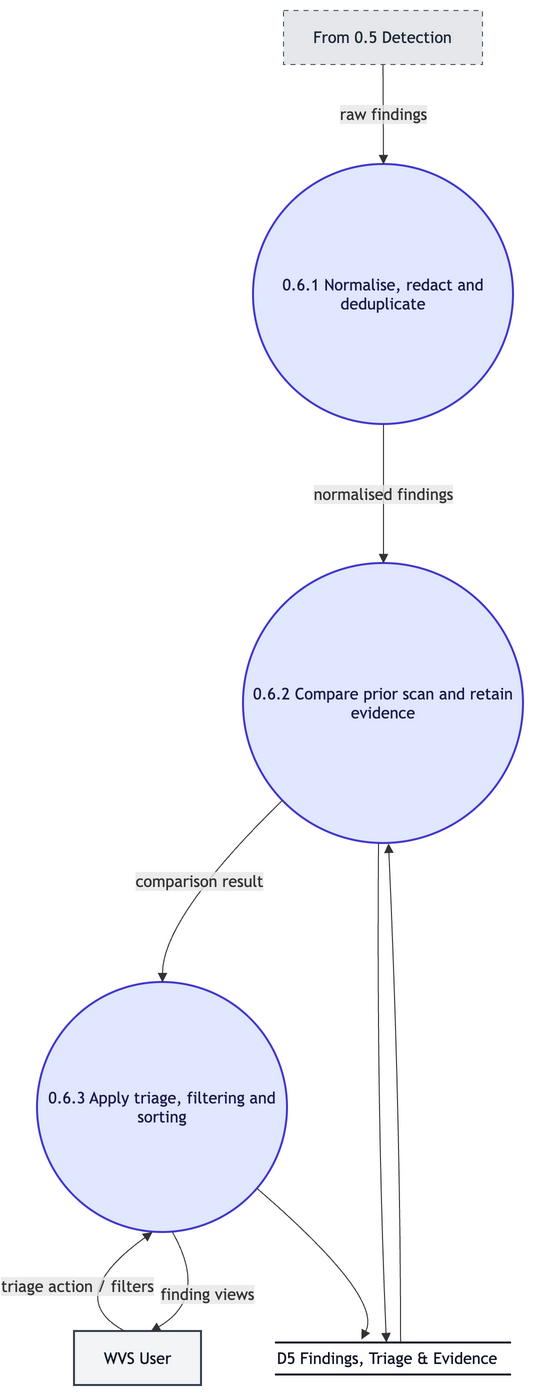
\includegraphics[width=0.94\textwidth,height=0.75\textheight,keepaspectratio]{mermaid/png/f.6.png}
    \caption{Level 2 DFD for 0.6 Findings Management}
    \label{fig:f6}
\end{figure}

\newpage
\subsubsection{0.7 Reporting \& Export}

Process $0.7$ is decomposed into completed scan selection, report template assembly, and export dispatch. Process 0.7.1 retrieves scan metadata from D4, Process 0.7.2 assembles the template, filters and limitations and the findings, triage and evidence from D5, and Process 0.7.3 generates export files (PDF/CSV) and triggers SMTP notifications.

\begin{figure}[H]
    \centering
    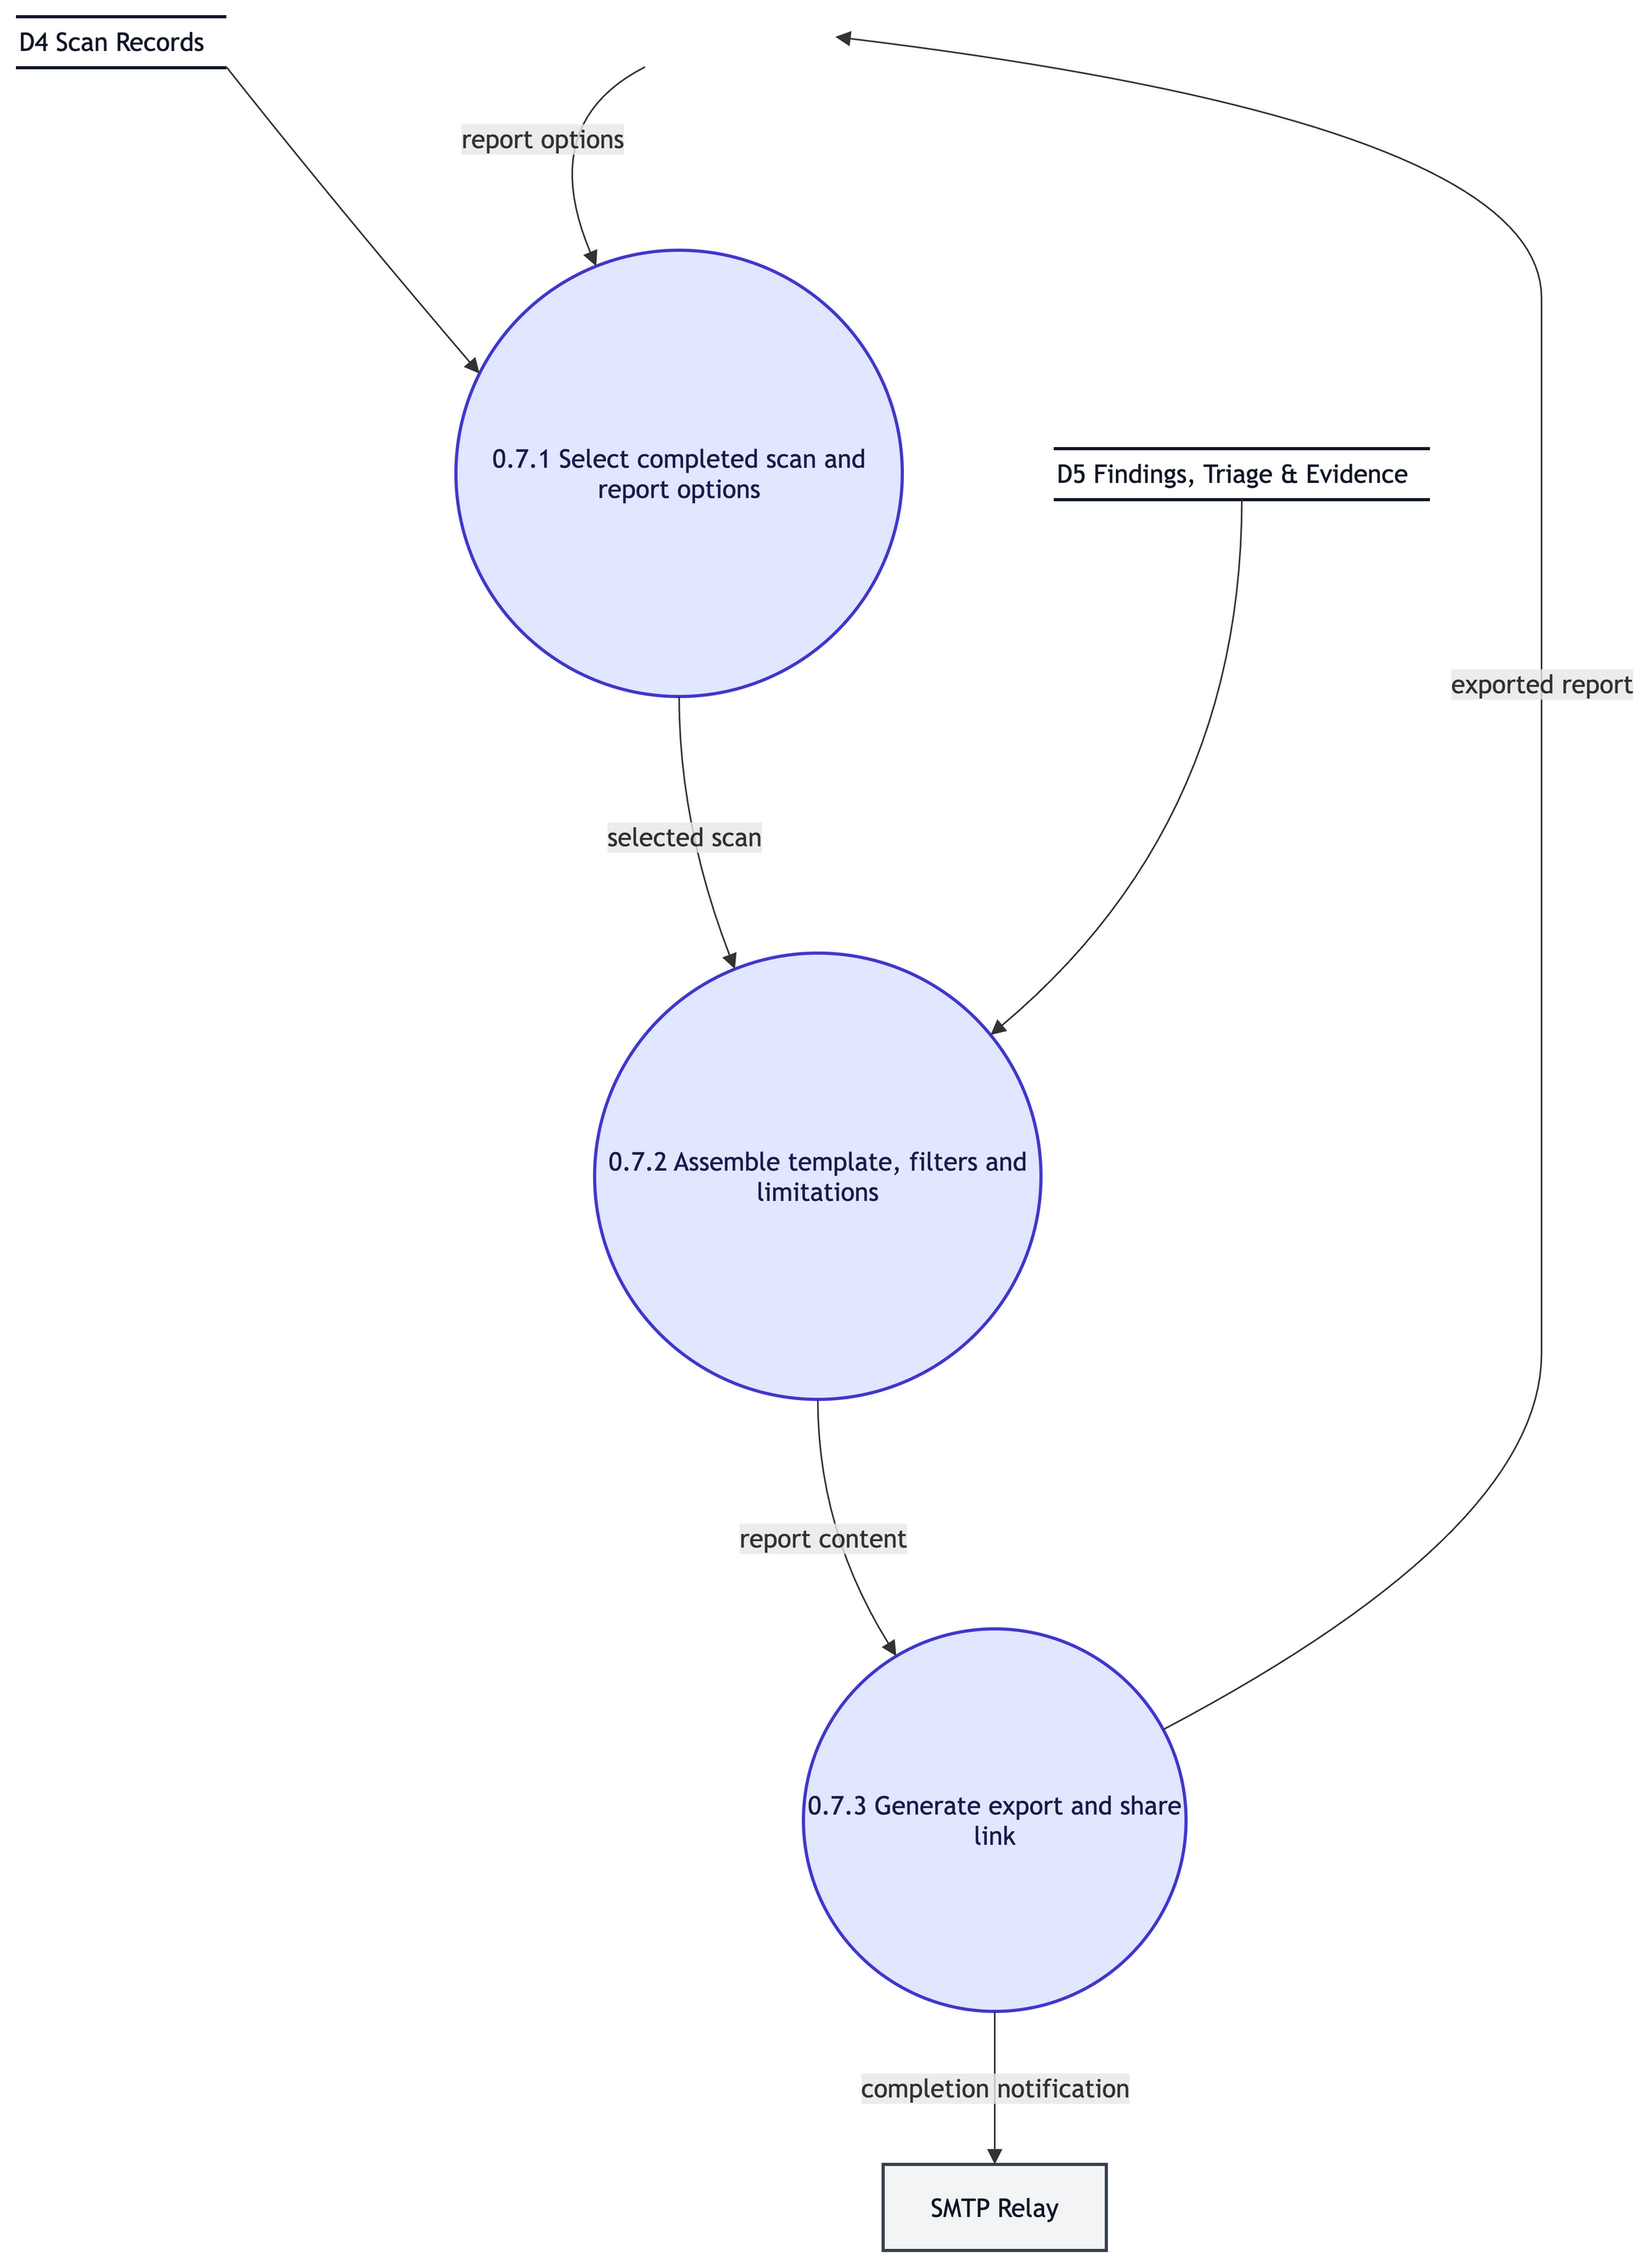
\includegraphics[width=0.94\textwidth,height=0.75\textheight,keepaspectratio]{mermaid/png/f.7.png}
    \caption{Level 2 DFD for 0.7 Reporting \& Export}
    \label{fig:f7}
\end{figure}

\subsubsection{0.8 Safety, Auditing \& Administration}

Process $0.8$ is decomposed into scope/blocklist verification, IP re-resolution \& rate limiting, and request dispatch. Process 0.8.1 checks requests against D2 policies. Process 0.8.2 performs fresh DNS checks to prevent SSRF, and Process 0.8.3 logs dispatches to D6 Append-only Audit Ledger.

\begin{figure}[H]
    \centering
    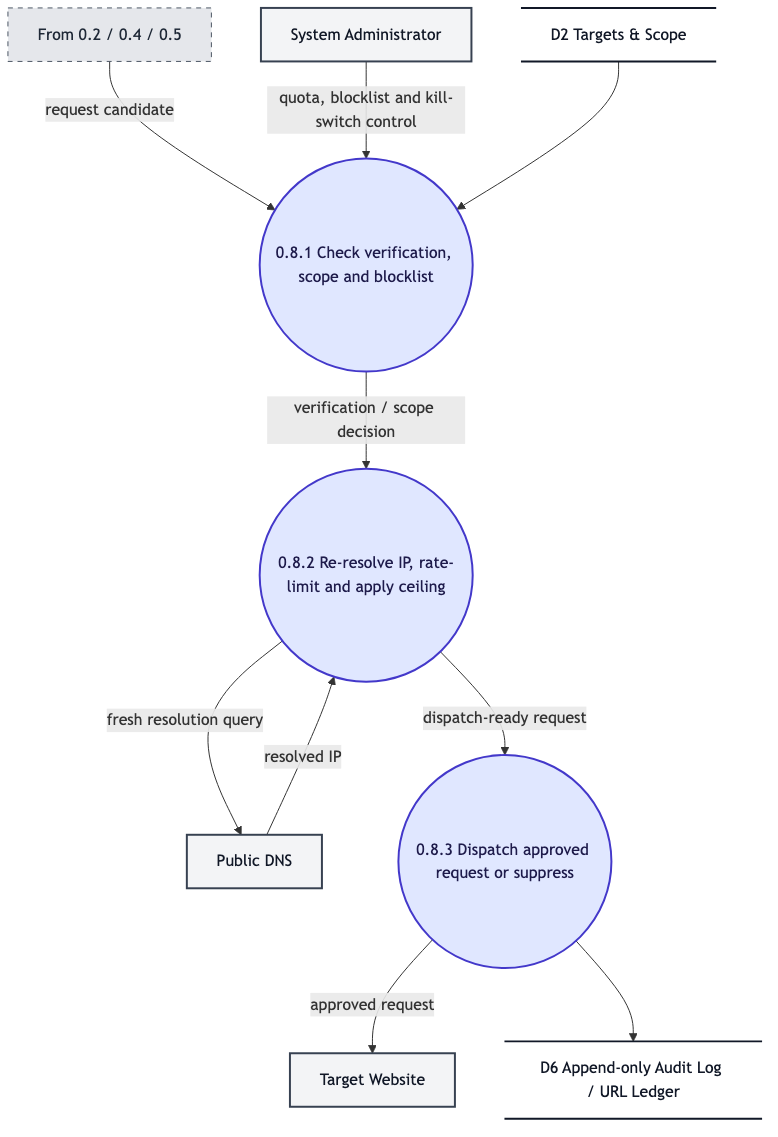
\includegraphics[width=0.94\textwidth,height=0.75\textheight,keepaspectratio]{mermaid/png/f.8.png}
    \caption{Level 2 DFD for 0.8 Safety, Auditing \& Administration}
    \label{fig:f8}
\end{figure}

\newpage
\section{Core Modules}

This section explains the main functional modules of the Website Vulnerability Scanner. Each module is responsible for a specific part of the scanning process, from user login and target verification to vulnerability detection and report generation.

\subsection{0.1 User Authentication \& Access Control}
This module manages user login, account registration, organisation onboarding, active sessions, and multi-factor authentication. It also helps protect user accounts by tracking login attempts and restricting access after repeated failures.
\begin{itemize}[noitemsep]
    \item \textbf{Functions}: Register users, verify login credentials and MFA, generate session tokens (JWT), record login activity, and apply account lockout when required.
\end{itemize}

\subsection{0.2 Target Management \& Authorisation}
This module allows users to register the websites or domains they want to scan and define the permitted scanning scope. It also verifies that the user has permission to scan the target using DNS TXT records or well-known verification files.
\begin{itemize}[noitemsep]
    \item \textbf{Functions}: Register targets and scan scope, generate verification tokens, validate DNS TXT or well-known proofs, and store scope rules.
\end{itemize}

\subsection{0.3 Scan Configuration \& Execution}
This module manages the configuration and execution of vulnerability scans. It checks whether the selected scan settings are valid, verifies user limits, schedules scan jobs, and keeps track of each stage of the scan.
\begin{itemize}[noitemsep]
    \item \textbf{Functions}: Validate scan profiles and quotas, queue or schedule scan jobs, manage scan execution and checkpoints, and store information required to reproduce a scan.
\end{itemize}

\subsection{0.4 Discovery (Crawling)}
This module explores the authorised website to identify possible attack surfaces such as links, forms, API endpoints, and dynamically generated JavaScript content. The crawler follows the limits and scope defined for the scan.
\begin{itemize}[noitemsep]
    \item \textbf{Functions:}\newline
    Load scope and crawling limits, discover links and sitemap entries, render JavaScript content, remove duplicate results, and send candidates to the Scope Guard for validation.
\end{itemize}

\subsection{0.5 Vulnerability Detection}
This module checks the discovered website components for security weaknesses. It performs passive checks on responses and headers, carries out safe active tests only on authorised targets, and uses external security databases to identify known vulnerabilities.
\begin{itemize}[noitemsep]
    \item \textbf{Functions}: Perform passive response checks, prepare safe active vulnerability tests, and check component versions using OSV and EPSS APIs.
\end{itemize}

\subsection{0.6 Findings Management}
This module processes the raw results produced during a scan and converts them into clear findings. It removes or hides sensitive information, compares findings with previous scans, and organises the results based on their severity and status.
\begin{itemize}[noitemsep]
    \item \textbf{Functions}: Normalise and redact findings, compare results with previous scan evidence, apply triage rules, filter findings, and sort them by severity.
\end{itemize}

\subsection{0.7 Reporting \& Export}
This module converts completed scan results into readable reports for both technical and non-technical users. It also supports exporting scan information and notifying users when a scan is complete.
\begin{itemize}[noitemsep]
    \item \textbf{Functions}: Select completed scans, prepare report templates and supporting evidence, generate PDF or CSV exports and share links, and send completion notifications through SMTP.
\end{itemize}

\subsection{0.8 Safety, Auditing \& Administration}
This module ensures that scans remain within the approved scope and follow the required safety rules. It checks target verification, blocks restricted destinations, re-checks IP addresses to reduce SSRF and TOCTOU risks, limits request rates, and records scanning activity for auditing.
\begin{itemize}[noitemsep]
    \item \textbf{Functions}: Verify target authorisation and scope blocklists, re-resolve IP addresses, apply rate limits, send approved requests, and maintain an append-only audit log.
\end{itemize}

\section{Structure Charts}

\subsection{Level 1 Structure Chart}
\subsubsection{Module Decomposition}

The structure chart is derived from the Level 1 and Level 2 DFDs using the structured design approach of Rajib Mall. The user-facing request routing is factored by transaction analysis into one action module per transaction path, and the scan pipeline ($0.3 \rightarrow 0.4 \rightarrow 0.5 \rightarrow 0.6$) is factored by transform analysis into an afferent branch, a transform centre, and an efferent branch. The Scope Guard modules (0.8) appear as shared library modules, with control couples (dotted arrows) carrying decisions such as approved/refused and lockout. Figure \ref{fig:structure_chart} illustrates the resulting module hierarchy.

\begin{figure}[H]
    \centering
    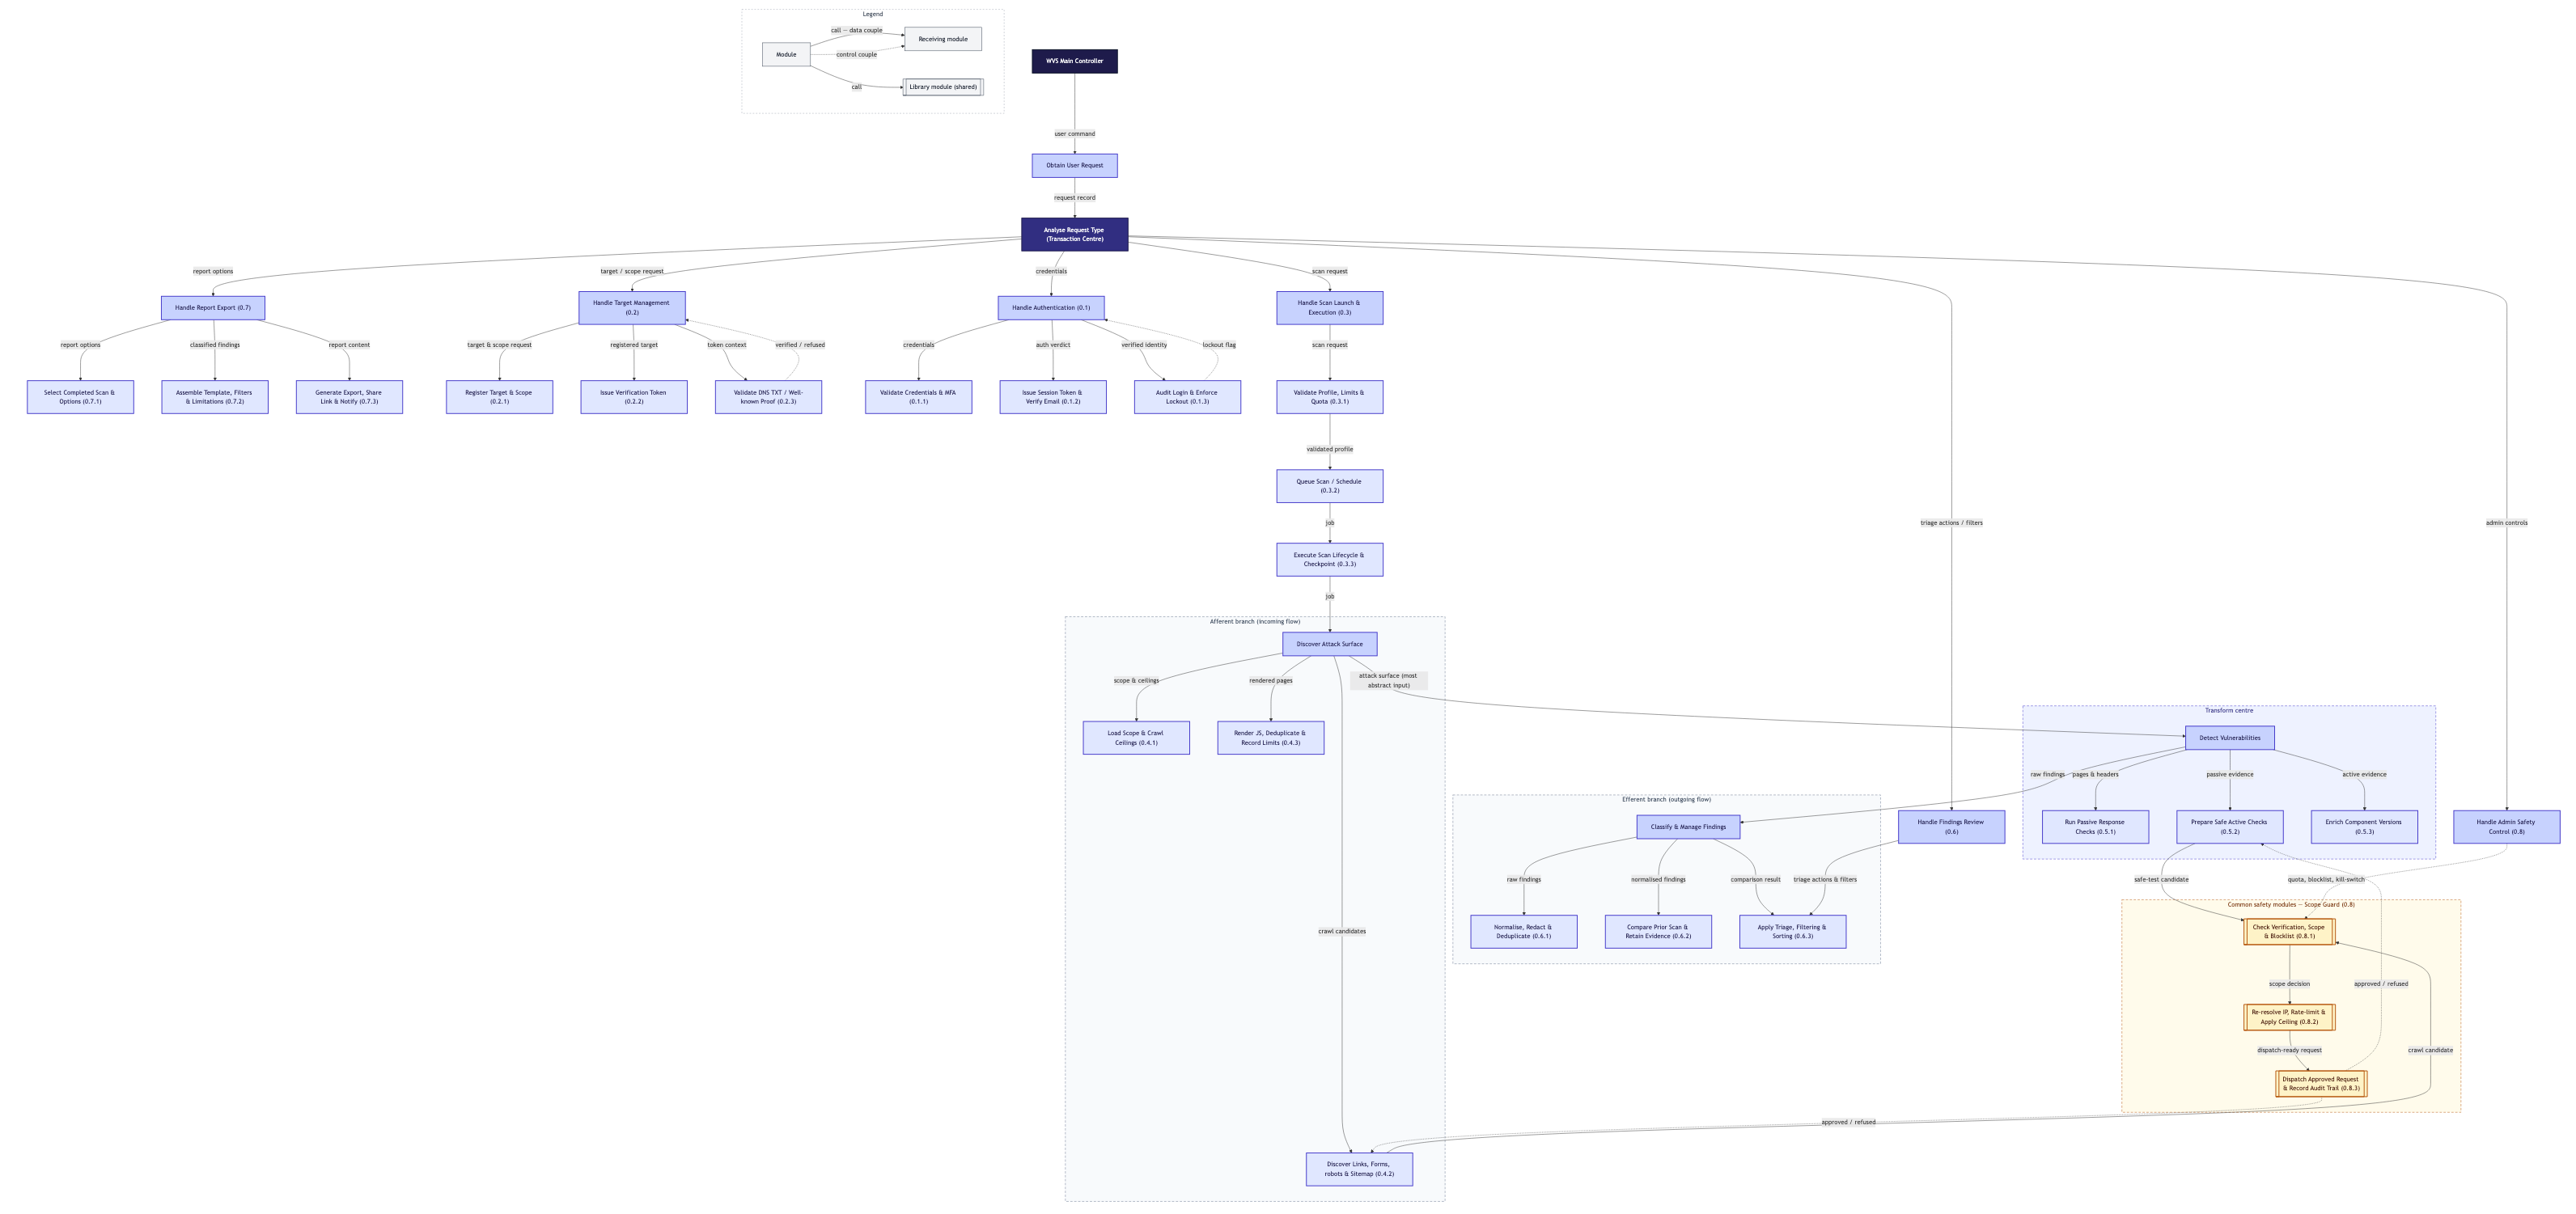
\includegraphics[width=\textwidth,height=0.55\textheight,keepaspectratio]{mermaid/png/structure-chart.png}
    \caption{Level 1 Structure Chart of the System}
    \label{fig:structure_chart}
\end{figure}

\end{document}
